% !TEX TS-program = pdflatex
% & -shell-escape

%%% CLASE DEL DOCUMENTO
\documentclass[letterpaper, 12pt]{article}

%%% PAQUETES BASE
\usepackage[T1]{fontenc}        
\usepackage[utf8]{inputenc}    
\usepackage{lmodern}
\usepackage[spanish, es-noshorthands]{babel}
\usepackage{comment}
\usepackage{textcomp}

%%% GEOMETRÍA DEL DOCUMENTO
\usepackage[top=3cm, bottom=2cm, right=2cm, left=2cm, headheight=15pt]{geometry}
\usepackage{multicol}
\usepackage{lscape}

%%% PAQUETES MATEMÁTICOS
\usepackage{amsmath, amsthm, amsfonts, latexsym, cancel}
\usepackage{amsbsy}
\usepackage{thmtools}
\usepackage{amssymb}
\usepackage{mathtools}

%%% PAQUETES PARA ESTILOS Y DISEÑO
\usepackage[dvipsnames]{xcolor}
\usepackage{tikz}
\usetikzlibrary{calc,shapes,shadows,decorations.pathmorphing}
\usepackage{mdframed}

%%% DEFINICIÓN DE COLORES
\definecolor{theoremBG}{RGB}{235,245,255}        % Fondo teorema más intenso
\definecolor{theoremBorder}{RGB}{210,225,250}    % Borde teorema más intenso
\definecolor{definitionBG}{RGB}{235,255,240}     % Fondo definición más intenso
\definecolor{definitionBorder}{RGB}{210,245,220} % Borde definición más intenso
\definecolor{remarkBG}{RGB}{255,240,230}         % Fondo observación más intenso
\definecolor{remarkBorder}{RGB}{250,220,205}     % Borde observación más intenso
\definecolor{easyBG}{RGB}{230,242,255}           % Fondo problema fácil más intenso
\definecolor{easyBorder}{RGB}{205,220,250}       % Borde problema fácil más intenso
\definecolor{mediumBG}{RGB}{255,240,225}         % Fondo problema medio más intenso
\definecolor{mediumBorder}{RGB}{250,220,205}     % Borde problema medio más intenso
\definecolor{hardBG}{RGB}{255,230,240}           % Fondo problema difícil más intenso
\definecolor{hardBorder}{RGB}{250,205,220}       % Borde problema difícil más intenso
\definecolor{exerciseBG}{RGB}{240,240,255}       % Fondo ejercicio más intenso
\definecolor{exerciseBorder}{RGB}{220,220,250}   % Borde ejercicio más intenso

%%% CONFIGURACIÓN DE ESTILOS TEOREMAS
\mdfdefinestyle{theoremstyle}{
    linecolor=theoremBorder,
    linewidth=0.4pt,                % Línea ligeramente más gruesa
    backgroundcolor=theoremBG!40,   % Fondo ligeramente más visible
    innertopmargin=10pt,
    innerbottommargin=10pt,
    innerleftmargin=10pt,
    innerrightmargin=10pt,
    skipabove=\topskip,
    skipbelow=\topskip,
}

% Aplicar el mismo patrón a los demás estilos
\mdfdefinestyle{definitionstyle}{
    linecolor=definitionBorder,
    linewidth=0.4pt,
    backgroundcolor=definitionBG!40,
    innertopmargin=10pt,
    innerbottommargin=10pt,
    innerleftmargin=10pt,
    innerrightmargin=10pt,
    skipabove=\topskip,
    skipbelow=\topskip,
}

\mdfdefinestyle{remarkstyle}{
    linecolor=remarkBorder,
    linewidth=0.4pt,
    backgroundcolor=remarkBG!40,
    innertopmargin=10pt,
    innerbottommargin=10pt,
    innerleftmargin=10pt,
    innerrightmargin=10pt,
    skipabove=\topskip,
    skipbelow=\topskip,
}

\mdfdefinestyle{easyproblemstyle}{
    linecolor=easyBorder,
    linewidth=0.4pt,
    backgroundcolor=easyBG!40,
    innertopmargin=10pt,
    innerbottommargin=10pt,
    innerleftmargin=10pt,
    innerrightmargin=10pt,
    skipabove=\topskip,
    skipbelow=\topskip,
}

\mdfdefinestyle{mediumproblemstyle}{
    linecolor=mediumBorder,
    linewidth=0.4pt,
    backgroundcolor=mediumBG!40,
    innertopmargin=10pt,
    innerbottommargin=10pt,
    innerleftmargin=10pt,
    innerrightmargin=10pt,
    skipabove=\topskip,
    skipbelow=\topskip,
}

\mdfdefinestyle{hardproblemstyle}{
    linecolor=hardBorder,
    linewidth=0.4pt,
    backgroundcolor=hardBG!40,
    innertopmargin=10pt,
    innerbottommargin=10pt,
    innerleftmargin=10pt,
    innerrightmargin=10pt,
    skipabove=\topskip,
    skipbelow=\topskip,
}

\mdfdefinestyle{exercisestyle}{
    linecolor=exerciseBorder,
    linewidth=0.4pt,
    backgroundcolor=exerciseBG!40,
    innertopmargin=10pt,
    innerbottommargin=10pt,
    innerleftmargin=10pt,
    innerrightmargin=10pt,
    skipabove=\topskip,
    skipbelow=\topskip,
}

%%% DEFINICIÓN DE TEOREMAS
\newtheorem{theorem}{Teorema}[section]
\newtheorem{corollary}{Corolario}[theorem]
\newtheorem{lemma}[theorem]{Lema}

\theoremstyle{definition}
\newtheorem{definition}{Definición}[section]

\theoremstyle{remark}
\newtheorem*{remark}{Observación}

\newtheorem{example}{Ejemplo}[section]
\newtheorem{easyproblem}{Problema}[section]
\newtheorem{mediumproblem}{Problema}[section]
\newtheorem{hardproblem}{Problema}[section]
\newtheorem{exercise}{Ejercicio}[section]

%%% APLICAR ESTILOS A LOS TEOREMAS
\surroundwithmdframed[style=theoremstyle]{theorem}
\surroundwithmdframed[style=theoremstyle]{corollary}
\surroundwithmdframed[style=theoremstyle]{lemma}
\surroundwithmdframed[style=definitionstyle]{definition}
\surroundwithmdframed[style=remarkstyle]{remark}
\surroundwithmdframed[style=theoremstyle]{example}
\surroundwithmdframed[style=easyproblemstyle]{easyproblem}
\surroundwithmdframed[style=mediumproblemstyle]{mediumproblem}
\surroundwithmdframed[style=hardproblemstyle]{hardproblem}
\surroundwithmdframed[style=exercisestyle]{exercise}

%%% ESTILO PARA DEMOSTRACIONES
\renewenvironment{proof}[1][\proofname]
    {\par\noindent\textit{#1.}\space}
    {\hfill$\square$\par\vspace{\baselineskip}}

%%% LENGUAJES DE PROGRAMACIÓN
\usepackage{verbatim}

%%% HIPERVÍNCULOS
\usepackage[
	breaklinks=true, 
	colorlinks=true, 
	linkcolor=blue,
	citecolor=blue, 
	urlcolor=gray
]{hyperref}
%% Divide los hipervínculos
\usepackage{xurl}

% Creative commons
\usepackage[scale=1.5]{ccicons}

%%% ESTILO DE REFERENCIAS
\usepackage{natbib}
\usepackage{apalike}

%%% ICONOS
\usepackage{marvosym}

%%% TEXTO GENERICO
\usepackage{lipsum}

%%% INDEX
\usepackage{imakeidx}
\makeindex[columns=3, title=Indice]

%Para paquetes .cvs
\usepackage{csvsimple}
\usepackage{xpatch}
\usepackage{etoolbox} % Para filtrar información en tablas.
\usepackage{booktabs} % Para hacer tablas bonitas desde un .csv

%Para escribir música
%\usepackage{musixtex}

%Estilo para programación.
\usepackage{listings}
\usepackage{color}
% http://paletton.com/#uid=7050t0kkJkJsntwoyp6gYgoddc4
%\usepackage[dvipsnames]{xcolor}
%	\definecolor{sec}{HTML}{DD5C14}
%	\definecolor{band}{HTML}{EE9C52}

% Paquete para pseudocódigo:
% \usepackage[Algoritmo]{algorithm}
\usepackage[spanish,onelanguage,ruled,vlined]{algorithm2e}
\usepackage[noend]{algpseudocode}

% Configuración para en ambiente de pseudocódigo:
\newcommand\mycommfont[1]{\footnotesize\ttfamily\textcolor{blue}{#1}}
\SetCommentSty{mycommfont}
\SetKwInput{KwInput}{Entrada}                
\SetKwInput{KwOutput}{Salida}             

% Ejemplo de pseudo código: 
\begin{comment}
\begin{algorithm}[H]
\DontPrintSemicolon
\BlankLine
\KwInput{Your Input}
\KwOutput{Your output}
\KwData{Testing set $x$}
$\sum_{i=1}^{\infty} := 0$ \tcp*{this is a comment}
\tcc{Now this is an if...else conditional loop}
\If{Condition 1}
{
Do something    \tcp*{this is another comment}
\If{sub-Condition}
{Do a lot}
}
\ElseIf{Condition 2}
{
Do Otherwise \;
\tcc{Now this is a for loop}
\For{sequence}    
{ 
loop instructions
}
}
\Else
{
Do the rest
}	
\tcc{Now this is a While loop}
\While{Condition}
{
Do something\;
}	
\caption{Example code}
\end{algorithm}
\end{comment}

% Definición de colores:
\definecolor{mygreen}{rgb}{0,0.6,0}
\definecolor{mygray}{rgb}{0.5,0.5,0.5}
\definecolor{mymauve}{rgb}{0.58,0,0.82}
\definecolor{orange}{RGB}{255,127,0}

% Estilo para escribir código de programación en el documento:
\renewcommand{\lstlistingname}{Código}
\lstset{ 
	keywordstyle=\color{blue},                % keyword style.	
	basicstyle=\footnotesize\ttfamily,        % size of fonts used for the code.
	commentstyle=\color{mygreen}\ttfamily,    % comment style.
	stringstyle=\color{mymauve},     % string literal style.
	backgroundcolor=\color{gray!5},          % choose the background color.
	rulecolor=\color{gray!5},                % border of the console.
	upquote=true,
	numbers=left, numberstyle=\tiny\color{gray}, stepnumber=1, numbersep=8pt, 
	% Formato de numeración.
	showstringspaces=false,
	breaklines=true,                 % automatic line breaking only at whitespace.
	frameround=ftff,
	frame=single,
	belowcaptionskip=-1.4em,
	belowskip=0em,
	aboveskip=-1.4em,
	captionpos=b,                    % sets the caption-position to bottom.
	escapeinside={\%*}{*)},          % if you want to add LaTeX within your code.
	literate={á}{{\'a}}1 {ã}{{\~a}}1 {é}{{\'e}}1 {í}{{\'i}}1 {ú}{{\'u}}1  {ó}{{\'o}}1,
}
% Ejemplo de  entorno de programación:
\begin{comment}
\begin{changemargin}{1.5cm}{1.5cm}
\begin{lstlisting}[language=python, caption={My caption},captionpos=b]
In [1]: logstart historia.py
\end{lstlisting}
\end{changemargin}
\end{comment}

% Gráficos, animaciones y diagramas.

\usepackage[all,color,dvips]{xy}
\usepackage{graphicx}
\DeclareGraphicsExtensions{.pdf,.png,.jpg}
%\usepackage{transparent}
\usepackage{eso-pic}



\usepackage{animate}
\usepackage {pst-solides3d}
\usepackage{pstricks}
\usepackage{pst-grad}
\usepackage{pst-3dplot}
\usepackage{pst-plot}
\usepackage{psfrag,pst-node} % Diagramas de Flujo
% \usepackage{pstcol} % Color para los Diagramas

% Paquetes para escribir expresiones matemáticas.
\usepackage{amsmath, amsthm, amsfonts, latexsym,cancel}
\usepackage{amsbsy}
\usepackage{thmtools}
\usepackage{amssymb}
\usepackage{xargs}
\usepackage{cancel} %Para tachar en formulas.
\usepackage{chemfig} % Fórmulas Químicas.
\usepackage[version=3]{mhchem}
\usepackage{epic,carom}
\usepackage{siunitx} % Para escribir unidades métricas. 

%Paquetes para tablas.
\usepackage{array} % Paquete para el diseño de tablas. 
\usepackage{multirow} % Para poder unir filas en las tablas
\usepackage{colortbl} % Para colorear tablas
\usepackage{longtable} % Controla el largo de la tabla
\usepackage{rotating} % Rotar tablas

% Maxima.
%\usepackage[amsmath]{maxiplot}

% Insertar etiquetas a las imágenes.
\usepackage{caption}[2013/02/03]
\usepackage{subcaption}
%Ejemplo de entorno de imagen con subcations:
%\begin{figure}
%\begin{minipage}[b]{.5\linewidth}
%  \centering\rule{2cm}{2cm}
% \subcaption{Primera subfigura}\label{fig:1a}
%\end{minipage}%
%\begin{minipage}[b]{.5\linewidth}
%  \centering\rule{2cm}{2cm$\BB$}
% \subcaption{Segunda subfigura}\label{fig:1b}
%\end{minipage}
%\caption{Figura con subfiguras}\label{fig:1}
%\end{figure}

% Tipo de letra del documento.
\usepackage{mathptmx}                 
\usepackage[scaled=.90]{helvet}         
\usepackage{courier}                
\usepackage{dsfont} 

% Numeración de las ecuaciones.
\usepackage{enumerate}
\numberwithin{equation}{section}

%Para partir enumeración.
\usepackage{enumitem}

% Espacio de líneas.
\linespread{1.2}
\usepackage{xspace} %Espacios después de los comandos.

% ARGUMENTOS VARIABLES
\usepackage{xargs}

% Lógica booleana para definir nuevos comandos:
\usepackage{ifthen}

% Example de comando usando el paquete ifthen:
\newcommand{\printTrueOrFalse}[1]
{
	\ifthenelse{\equal{#1}{true}}{TRUE}{}
	\ifthenelse{\equal{#1}{false}}{FALSE}{}
}

% NOTAS
\setlength {\marginparwidth }{2cm}
\usepackage[colorinlistoftodos, prependcaption]{todonotes}
\newcommandx{\note}[2][1=]{
	\todo[
	linecolor=green,
	backgroundcolor=green!25,
	bordercolor=green,#1]{#2}
}


% Definición de comandos matemáticos:
\newcommand{\KK}{\mathbb{K}} %Un cuerpo cualquiera.
\newcommand{\EE}{\mathcal{E}} %Espacio euclidiano.
\newcommand{\FF}{\mathbb{F}} %Campo comutativo.
\newcommand{\HH}{\mathbb{H}} %Semiespacio real superior.
\newcommand{\RR}{\mathbb{R}} %Números Reales.
\newcommand{\ZZ}{\mathbb{Z}} %Número Enteros.
\newcommand{\NN}{\mathbb{N}} %Numero Natureles.
\newcommand{\NNO}{\mathbb{N}_{_0}} %Numero Natureles.
\newcommand{\QQ}{\mathbb{Q}} %Números Racionales.
\newcommand{\CC}{\mathbb{C}} %Números Complejos
\newcommand{\RP}{\mathbb{RP}} %Plano proyectivo.
\newcommand{\A}{\mathcal{A}} %Atlas.
\newcommand{\B}{\mathcal{B}} %Atlas.
\newcommand{\BB}{\mathbb{B}} %Atlas.
\newcommand{\E}{\mathbb{E}} %Variedad Euclidiana.
\newcommand{\VV}{\mathbb{V}} %Espacio Vectorial V.
\newcommand{\hw}{\hspace{0.3cm}} %Espacio de 0.2cm.
\newcommand{\J}{\pmb{J}} %Jacobiano.
\newcommand{\ck}{\;_{\widetilde{C}^{k}}\,}  %Relación C^k - compatibles.
\newcommand{\cl}{\;_{\widetilde{C}^{l}}\,}  %Relación C^l - compatibles.
\newcommand{\cp}{\;_{\widetilde{p}}\,}  %Relación p - relacionados.
\newcommand{\ckr}{\;_{\widetilde{C}^{r}}\,} %Relacion C^r - compatibles.
\newcommand{\G}{\;_{\widetilde{G}}\;} 
\newcommand{\Ck}{_{\widetilde{C}^{k}}\,}
\newcommand{\C}{\mathcal{C}}
\newcommand{\cd}{\;|\;}
\newcommand{\fl}{f\hspace{0.0499em}l}
\newcommand{\fii}{f\hspace{0.03em}i}

% Comandos para que el csvsimple reconozca las tablas
\newcommand{\standardroman}[1]{\romannumeral\value{#1}}
\makeatletter
\xpatchcmd{\csv@breakline@kernel}{\roman}{\standardroman}{}{}
\xpatchcmd{\csv@current@col}{\roman}{\standardroman}{}{}
\xpatchcmd{\set@csv@autohead}{\roman}{\standardroman}{}{}
\xpatchcmd{\set@csv@head}{\roman}{\standardroman}{}{}
\xpatchcmd{\set@csv@nohead}{\roman}{\standardroman}{}{}
\makeatother


\def\SS{\mathbb{S}} %Esfera.
\def\TT{\mathbb{T}} %Toro.
\def\AA{\mathbb{A}} %Módulo A.
\def\LL{\mathcal{L}} %Familia de rectas. 
\def\PP{\mathcal{P}} %Familia de planos.


%Definición de operadores.
\DeclareMathOperator{\sen}{sen\,} %Función seno.
\DeclareMathOperator{\senh}{senh\,} %Función seno hiperbólico.
\DeclareMathOperator{\sech}{sech\,} %Función secante hiperbólico.
\DeclareMathOperator{\rot}{rot\,} %Rotacional.
\DeclareMathOperator{\dive}{div\,} %Divergencia.
\DeclareMathOperator{\nulo}{nul\,} %Nulo.
\DeclareMathOperator{\im}{img} %Imagen.
\DeclareMathOperator{\id}{id} %Función identidad.
\DeclareMathOperator{\Tr}{Tr\,} %Traza. 
\DeclareMathOperator{\Crit}{Crit\,} %Cunjunto de puntos críticos.
\DeclareMathOperator{\md}{\;mod} %Modulo.
\DeclareMathOperator{\ord}{ord} %Orden.
\DeclareMathOperator{\mcd}{mcd} %Máximo común divisor.
\DeclareMathOperator{\mcm}{mcm} %Mínimo común múltiplo
\DeclareMathOperator{\Gr}{Gr} %Gráfica.
\DeclareMathOperator{\orb}{orb} %Orbita.
\DeclareMathOperator{\dif}{dif} %Conjunto de difeomorfismos.
\DeclareMathOperator{\GL}{GL} %Grupo Especial Lineal 
\DeclareMathOperator{\Int}{Int} %Interior de un grupo 
\DeclareMathOperator{\sgn}{sgn} %Signo de una permutación
\DeclareMathOperator{\sop}{sop} %Soporte de una partición
\DeclareMathOperator{\dom}{dom} %Domino
\DeclareMathOperator{\ran}{ran} %Rango
\DeclareMathOperator{\Arg}{Arg} %Argumento de un número complejo
\DeclareMathOperator{\End}{End} %Endomorfismos
\DeclareMathOperator{\vol}{vol} %Volumen
\DeclareMathOperator{\Hom}{Hom} %Homomorfismos
\DeclareMathOperator{\Der}{Der} %Derivaciones
\DeclareMathOperator{\SO}{SO} %Grupo ortogonal especial
\DeclareMathOperator{\U}{U} %Grupo unitario
\DeclareMathOperator{\SU}{SU} %Grupo unitario especial
\DeclareMathOperator{\SL}{SL} %Grupo lineal especial
%\DeclareMathOperator{\tr}{tr} %Traza de una matriz
\DeclareMathOperator{\diag}{diag} %Matriz diagonal
\DeclareMathOperator{\Lie}{Lie} %Matriz diagonal
\DeclareMathOperator{\proy}{proy} %Matriz diagonal
\DeclareMathOperator{\card}{card} %Cardinal de un conjunto
\DeclareMathOperator{\instab}{instab} %Inestabilidad de un AC.
\DeclareMathOperator{\gen}{gen} %Generador.
\DeclareMathOperator{\Colu}{Col} %Columna.
\DeclareMathOperator{\vari}{var} %Varianza.
\DeclareMathOperator{\adj}{adj} %Varianza.
\DeclareMathOperator*{\argMin}{arg\, min} % Argumento minimal.
\DeclareMathOperator{\Jac}{\pmb{J}} % Jacobiano


% LISTA DE COMANDOS GENERALIZADOS:
% Comando nuevo para calcelar con diferentes colores.
\newcommand{\Cancel}[2][black]{\renewcommand\CancelColor{\color{#1}}\cancel{#2}}

% Comando para una lista de puntos. 
\newcommandx{\points}[3][1=0, 3=n]{#2_{_{#1}},\ldots,#2_{_{#3}}} 

% COMANDOS MATEMÁTICOS SIMPLES:

% Función del argumento mínimo:
\newcommand*\argmin[1]{\argMin_{#1}} 

% Insertar fondo de página en el documento:
\newcommandx{\BackgroundPic}[1]{
	\put(-3,0){
		\parbox[b][\paperheight]{\paperwidth}{%
			\vfill
			\centering
			{\includegraphics[width=\paperwidth,height=\paperheight]{#1}}%
			%{\transparent{#2}\includegraphics[width=\paperwidth,height=\paperheight]{#1}}% Está linea solo funciona con pfdtex
			\vfill
}}}

% DEFINICIÓN DE NUEVOS ACENTOS:

% Acento de arco:
\DeclareFontFamily{OMX}{yhex}{}
\DeclareFontShape{OMX}{yhex}{m}{n}{<->yhcmex10}{}
\DeclareSymbolFont{yhlargesymbols}{OMX}{yhex}{m}{n}
\DeclareMathAccent{\arco}{\mathord}{yhlargesymbols}{"F3}


% Acentos:
\begin{comment}
    $\arco{AB}$ $\widehat{ABC}$
\end{comment}

% Comandos para notas:
\usepackage[colorinlistoftodos,prependcaption]{todonotes}
\newcommandx{\unsure}[2][1=]{\todo[linecolor=red,backgroundcolor=red!25,bordercolor=red,#1]{#2}}
\newcommandx{\change}[2][1=]{\todo[linecolor=blue,backgroundcolor=blue!25,bordercolor=blue,#1]{#2}}
\newcommandx{\info}[2][1=]{\todo[linecolor=green,backgroundcolor=green!25,bordercolor=green,#1]{#2}}
\newcommandx{\improvement}[2][1=]{\todo[linecolor=Plum,backgroundcolor=Plum!25,bordercolor=Plum,#1]{#2}}
\newcommandx{\thiswillnotshow}[2][1=]{\todo[disable,#1]{#2}}

% Renombrado comandos: 

\renewcommand\figureautorefname{Figura}
\renewcommand\pageautorefname{pagína}
\renewcommand\algorithmautorefname{Algoritmo}
\renewcommand\theoremautorefname{Teorema}


% Comando para hyperefereces:
\newcommand{\sref}[2]{\hyperref[#2]{#1 \ref*{#2}}}

%Paquetes para el diseño del encabezado.
\usepackage{fancyhdr}
\usepackage{fancyvrb}
%\usepackage{parskip} % Quita la indentación inicial de los parráfos. 

\pagestyle{fancy}
\renewcommand{\sectionmark}[1]{\markboth{#1}{}} % Quita la numeración de los capitulos en el encabezado.
\fancyhf{}
%\fancyhead[LE]{\nouppercase{\small\textit \thepage}\small\it{/Tensor Geométrico}} %Ubica el título del libro en pares.
\fancyhead[RO]{\nouppercase{\small\textit\leftmark \,/}{\small\textit \thepage}} %Ubica el título del capitulo en impares.
\fancypagestyle{plain}{\fancyhead{}}
\renewcommand{\headrulewidth}{0pt}

%Corrige la separación de palabras.
%\usepackage[none]{hyphenat} 
\hyphenation{corres-pondencia equiva-lente geo-metría posibi-lidad axio-mas}

%Líneas huerfanas.
\tolerance 1414
\hbadness 1414
%\emergencystretch 1.5em
\hfuzz 0.3pt
\vfuzz \hfuzz
%\raggedbottom
%Lo anterior está en prueba
\clubpenalty=1000
\widowpenalty=1000

\def\changemargin#1#2{\list{}{\rightmargin#2\leftmargin#1}\item[]}
\let\endchangemargin=\endlist

\setlength{\parindent}{0cm}
% Define el espacio entre parrafos. 
\setlength{\parskip}{2mm}

% Espacio entre teorema y demostración:
\usepackage{etoolbox}

% Árboles
\usepackage{qtree}

% \definecolor{micolor}{RGB}{255,255,240}
% \pagecolor{micolor}

 

\begin{document}
	\thispagestyle{empty}
	\begin{center}
		{\Large\textbf{GENERALIZACIÓN DEL JUEGO LIGHT 
		OUT A UN GRAFO DE MÚLTIPLES ESTADOS}} \\
		\bigskip Alejandro Sánchez Yalí 
		\\ {\footnotesize\emph{Facultad de Ciencias Exactas y Naturales,
		 Universidad de Antioquia, Medellín, Colombia}.\\
		\textbf{E-mail:} alejandro.sanchezy@udea.edu.co}\\
		{\footnotesize\today.}\\\vspace{0.1cm}
		{\small\ccbysa}
	\end{center}
	
\begin{section}{Introducción}

\text{Light Out} es un juego producido por Tiger Electronics que consta de 
una cuadrícula de botones de cinco por cinco; cada botón tiene una bombilla 
indicadora que puede estar encendida o apagada. Al presionar un botón, las 
bombillas de los botones adyacentes a él en filas y columnas, si existen, 
cambian de estado. La finalidad del juego es, dada un configuración inicial de 
bombillas encendidas y apagadas, ir 
pulsando los botones necesarios hasta conseguir apagar todas las bombillas.  

En 1998, Anderson y Feil (\cite{anderson1998turning}) resolvieron el juego 
original empleando álgebra lineal. Han aparecido varios artículos que han estudiado el problema con diferentes variaciones, tales como, \cite{ barua1996sigma, eriksson2001note,  fleischer2013survey, hunziker2004chebyshev, martin2001two,	scherphuis2014mathematics, sutner2000sigma}. El objetivo aquí, será exponer la solución planteada por Feil y Anderson en 1998 (\cite{anderson1998turning}); además de generalizar el problema a un 
grafo con múltiples estados en $\ZZ_{_p}$ y diferentes velocidades de cambio por nodo, junto con algunos de los resultados presentados por Giffen, Alexander, y D. Parker en 2009 (\cite{giffen2009generalizing}).

\begin{section}{Light Out y los sistemas lineales binarios}
Feil y Anderson en \cite{anderson1998turning}, resolvieron el juego original que consiste de una cuadrícula de cinco por cinco; para esto, hicieron uso del Álgebra Lineal con todas las operaciones hechas bajo módulo 2; lo que permite encontrar una estrategia completa para apagar todas las bombillas frente a cualquier configuración inicial del juego. \info{¿Dejar la cantidad mínima de bombillas encendidas?} Ellos, consideraron que el estado de cada una de las bombillas es representado por un elemento del conjunto $\ZZ_{_2}$, el campo de enteros módulo 2; en el cual, el $1$ significa que la bombilla está encendida, y el 2, que está apagada. El estado de cada bombilla ubicada en la $i$-ésima fila y la $j$-ésima columna, se representa por $b_{_{ij}}\in \ZZ_{_2}$, que es una entradadel vector columna $\pmb{b}$ de orden $25\times 1$, ordenado de la siguiente 
forma:
\begin{equation}
\pmb{b}= (b_{_{11}}, b_{_{12}}, b_{_{12}},\dots, b_{_{15}},  b_{_{21}},\dots, 
b_{_{55}})^{\top}.
\end{equation}
Cada vector $\pmb{b}\in \ZZ_{2}^{25}$ representa una \textbf{configuración} del 
juego. Por ejemplo, 
\[\pmb{b}=(1,1,0,0,1,0,0,0,0,0,0,0,0,0,0,0,0,0,0,0,1,0,0,0,1)^{\top}\] donde 
$0$ 
indica apagado y $1$ encendido, describe una situación como en la figura 
\ref{fig:lightout}.

\begin{figure}[t!]
\centering
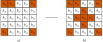
\includegraphics[scale=1]{Figures/ligthout1}
\caption{Representación de la configuración 	
$\pmb{b}=(1,1,0,0,1, 0,0,0,0,0, 0,0,0,0,0, 0,0,0,0,0,  1,0,0, 0, $ $1)^{\top}$ 
para el juego de Light Out $5\times 5$ y cómo cambia cuando se pulsa el botón 
$b_{_{33}}$.}
\label{fig:lightout}
\end{figure}
Cuando se modifica el estado de una bombilla, cambia el vector de 
configuración, 
sumando un vector de $\ZZ_{2}^{25}$ con $1$ en las posiciones 
correspondientes a las bombillas adyacentes a ésta en filas y columnas,  y cero 
en los demás casos. Por ejemplo, en la figura \ref{fig:lightout}, el estado 
dado 
por $\pmb{b}=(1,1,0,0,1,   0,0,0,0,0,   0,0,0,0,0, $ $ 0,0,0,0,0,  
1,0,0,0,1)^{\top}$ se transforma en la configuración $(1,1,0,0,1,   
0,0,1,0,0,   0,1,1,1,0,  0,0,1,0,0, $ $  1,0,0,0,1)^{\top}$, que se produce cuando 
a $\pmb{b}$ se le suma el vector $(0,0,0,0,0,   0,0,1,0,0,   0,1,1,1,0,  
0,0,1,0,0,$ $  0,0,0,0,0)^{\top}$.



Por otro lado, una \textbf{estrategia} se entenderá como un 
vector $-\pmb{x}$  de $\ZZ_{2}^{25}$ donde  $x_{_{ij}}$ es $1$ si la bombilla 
$(i, j)$ es alterada y cero en los demás casos. 

Note con detenimiento que la estrategia ganadora $\pmb{x}$ cumple las 
ecuaciones:
\begin{eqnarray*}
	b_{_{11}} &=& (x_{_{11}}+x_{_{12}}+x_{_{21}})\mod 2,\\
	b_{_{12}} &=& (x_{_{11}}+x_{_{12}}+x_{_{13}}+x_{_{22}}) \mod 2,\\
	b_{_{13}} &=& (x_{_{12}}+x_{_{13}}+x_{_{14}}+x_{_{23}}) \mod 2,\\
	&\vdots & \\
	b_{_{54}} &=& (x_{_{44}}+x_{_{53}}+x_{_{54}}+x_{_{55}}) \mod 2,\\
	b_{_{55}} &=& (x_{_{54}}+x_{_{45}}+x_{_{55}}) \mod 2.
\end{eqnarray*}

Dicho sistema puede escribirse en la forma $A \pmb{x} = \pmb{b}$, donde 
los arreglos tienen dimensiones $25\times 25$, $25\times 
1$ y 
$25\times 1$ respectivamente. De manera m\'as precisa, $A$ está constituida por 
bloques; los cuales serán 
descritos a continuaci\'on:
\begin{equation}\label{A_clasico}
A=
\begin{bmatrix}
B & I & O & O & O  \\ 
I & B & I & O  & O \\
O & I & B & I & O  \\
O & O & I & B & I   \\
O & O & O & I & B   \\
\end{bmatrix}
\end{equation}

\begin{center}
	
	$B= 
	\begin{bmatrix}
	1 & 1 & 0 & 0 & 0  \\ 
	1 & 1 & 1 & 0  & 0 \\
	0 & 1 & 1 & 1 & 0  \\
	0 & 0 & 1 & 1 & 1   \\
	0 & 0 & 0 & 1 & 1   \\
	\end{bmatrix},\ 
	I=
	\begin{bmatrix}
	1 & 0 & 0 & 0 & 0  \\ 
	0 & 1 & 0 & 0  & 0 \\
	0 & 0 & 1 & 0 & 0  \\
	0 & 0 & 0 & 1 & 0   \\
	0 & 0 & 0 & 0 & 1   \\
	\end{bmatrix},\ 
	O=
	\begin{bmatrix}
	0 & 0 & 0 & 0 & 0  \\ 
	0 & 0 & 0 & 0  & 0 \\
	0 & 0 & 0 & 0 & 0  \\
	0 & 0 & 0 & 0 & 0   \\
	0 & 0 & 0 & 0 & 0   \\
	\end{bmatrix} $	
\end{center}

Recuerde de \'Algebra Lineal que dada una matriz $A$, el complemento ortogonal 
del espacio columna de $A$ es el espacio nulo izquierdo de $A$; y que 
tambi\'en, el 
complemento ortogonal del espacio fila de $A$ es el espacio nulo de $A$.

Observe que, el problema $A\pmb{x} = \pmb{b}$ es soluble sí y s\'olo sí,
$\pmb{b}$ 
es combinaci\'on lineal de las columnas de $A$; es decir, existe una estrategia 
ganadora $\pmb{x}$ sí y s\'olo sí, $\pmb{b}$ est\'a en el espacio 
columna de $A$. Sin embargo, si se nota que $A$ es sim\'etrica y que por ende, 
los 
espacios columna y fila de $A$ son iguales, se puede decir que existe una 
estrategia ganadora $\pmb{x}$ siempre y cuando ésta est\'e en el 
espacio fila de $A$; de manera equivalente, $\pmb{x}$ tiene que ser 
ortogonal a todo vector en el espacio nulo de $A$. Lo dicho, implica que se 
puede generar un criterio con el que se pueda verificar si dada una 
configuraci\'on inicial $\pmb{b}$ en el juego Lights Out, se puede o no, 
hallar una estrategia ganadora o soluci\'on $\pmb{x}$.

Empleando reducci\'on con operaciones elementales de fila, pero en $\ZZ_{_2}$, 
se puede hallar una base para el espacio nulo (espacio soluci\'on de $A 
\pmb{x} = \pmb{0}$). Dicha base tiene los elementos: $$\pmb{n} 
_{1}=(0,1,1,1,0,1,0,1,0,1,1,1,0,1,1,1,0,1,0,1,0,1,1,1,0)^{\top}$$
$$\pmb{n}_{2}=(1,0,1,0,1,1,0,1,0,1,0,0,0,0,0,1,0,1,0,1,1,0,1,0,1)^{\top}$$
Dada una configuraci\'on inicial $\pmb{b}$, se pueden apagar todas las 
luces, siempre y cuando se cumpla que,
\begin{equation}\label{condicion}
\pmb{b} \cdot \pmb{n} _{1} = \pmb{b} \cdot \pmb{n} _{2} = 0
\end{equation}
Cuando $\pmb{b}$ cumpla con la ecuación (\ref{condicion}), se puede usar el 
m\'etodo de Gauss-Jordan con operaciones m\'odulo 2, para hallar la soluci\'on 
de $ A\pmb{x} 
= 
\pmb{b}$. Cabe notar que, si $\pmb{x}$ es una soluci\'on, entonces los 
inversos aditivos de $\pmb{x}$,  
$\pmb{x}+\pmb{n}_{1}, \pmb{x}+\pmb{n}_{2}$ y 
$\pmb{x}+\pmb{n}_{1}+\pmb{n}_{2}$ en $\ZZ_{_2}$ son estrategias 
ganadoras.\info{¿Son todas las estrategias ganadoras}\\

Note que las bombillas también se pueden entender como nodos de un grafo, en 
donde hay una arista entre dos nodos (bombillas) si los estados de ambas son 
mutuamente dependientes. En efecto, la matriz $A$ del sistema 
$A\pmb{x}=\pmb{b}$ es realmente su matriz de adyacencia. Esta interpretación, 
da paso a generalizar el juego Light Out a un grafo no orientado, donde cada 
nodo va estar asociado con un estado caracterizado por algún elemento de 
$\ZZ_{n}$. 


\end{section}
\end{section}
\begin{section}{Light Out}
	
Un juego de Light Out es un arreglo de la forma $(G, \ZZ_{_n}, A, 
s_{_0})$ donde $G$ es un grafo finito con $m$ vértices $V(G)$ y 
aristas $E(G)$. El conjunto de vértices, es etiquetado con una 
\textbf{distribución inicial de estados} dada por la función $s_{_0}:V(G)\to 
\ZZ_{_n}$ y una \textbf{matriz de relación $A$}, tal que $A_{_{vw}}\in 
\ZZ_{_n}\setminus 
\{0\}$\info{¿Qué ocurre si es cero?} si $v=w$ o $vw\in E(G)$, y cero en los demás casos. Con fines 
didácticos, el conjunto de vértices $V(G)$ se identificará con el 
conjunto de número naturales $\{1,2, \dots, m\}$.

Si $s_{_{t-1}}$ es una \textbf{distribución de estados en el tiempo $t-1\in 
\NN_{_0}$}, cuando se \textbf{pulsa} un vértice $v$, todos los vértices $w$ que 
se encuentran relacionados con $v$ mediante la matriz $A$, cambian su estado de 
acuerdo con: 
\begin{equation}
s_{_t}(w) = (s_{_{t-1}}(w)+A_{_{wv}})\md(n).
\end{equation}
Recursivamente se tiene que,
\begin{equation}
s_{_{t}}(w)=(s_{_0}(w)+tA_{_{wv}})\md(n).
\end{equation}
Sea $\pmb{x}\in \ZZ_{p}^{m}$ donde la $v$ - ésima entrada $x_{_v}$ es el número 
de veces que se ha pulsado el vértice $v$ desde el momento inicial; por lo 
tanto, el estado del vértice $w$ en tiempo $t = \sum_{v\in V(G)}x_{_v}$ es: 
\begin{equation}
s_{_t}(w)=\left(s_{_0}(w)+\sum_{v\in V(G)}A_{_{wv}}x_{_v}\right)\md(n).
\end{equation}

Se dirá que un juego de Ligth Out es \textbf{soluble} si existe un 
$-\hat{\pmb{x}}$ tal que, para el tiempo $t = \sum_{v\in V(G)}\hat{x}_{_v}$ la 
distribución de estados sea $s_{_t}(w) = 0$ para todo $w \in V(G)$; es decir,
\begin{equation}
(\pmb{s}_{_0}-A\hat{\pmb{x}})\md(n) = 0,
\end{equation}
donde $\pmb{s}_{_0}$ es un vector columna dado por $(s_{_0}(1),\dots, 
s_{_0}(m))^{\top}$. Finalmente, con lo anterior se ha establecido el siguiente 
resultado:
\begin{theorem} Un juego Light Out $(G, \ZZ_{_n}, A, 
	s_{_0})$ es soluble sí y sólo sí, $A\pmb{x} = 
\pmb{s}_{_0}$ es soluble sobre $\ZZ_{_n}$.
\end{theorem}

\begin{example}\textbf{Light Out hexagonal 3 - 5 - 3.}
	Considere el grafo $G$ donde los vértices son las 19 casillas hexagonales 
	que se muestran en la figura \ref{fig:lightout2}. Las aristas, son 
	definidas 
	por los hexágonos adyacentes y los estados de cada casilla se toman en 
	$\ZZ_{_2}$ . Tomando la figura 2.a como configuración inicial del juego, 
	cada que se presiona una casilla, cambia ella y todas las casillas 
	adyacentes; en efecto, si se presiona la casilla $c_{_{10}}$, los cambios 
	de estado se dan en todas las casillas adyacentes incluyendo $c_{_{10}}$, 
	ver figura 2.b. 
	
	
	\begin{figure}[ht!]
		\centering
		
\includegraphics[scale=1]{Figures/ligthout2}
		\caption{Cuando se presiona la casilla $c_{_{10}}$, todas las casillas 
		adyacentes cambian su estado.}
		\label{fig:lightout2}
	\end{figure}
	
	
	La matriz $A$ que ayuda a modelar el juego Ligths Out hexagonal 3 - 5 - 3 es:
	\begin{equation}
	A = \left[\begin{array}{ccccc}
	D_{_3} & S_{_{34}} & O & O & O \\
	S_{_{34}}^{\top} & D_{_{4}} & S_{_{45}} & O & O \\
	O & S_{_{45}}^{\top} & D_{_{5}} & S_{_{45}}^{\top} & O \\
	O & O & S_{_{45}} & D_{_4} & S_{_{34}}^{\top} \\
	O & O & O & S_{_{34}} & D_{_3} \\
	\end{array}\right]
	\end{equation}
	donde $D_{_n}$ es una  matriz  de orden $n\times n$ y tridiagonal de unos. 
	Las matrices $S_{_{34}}$ y $S_{_{45}}$ son bidiagonales de unos. 
	Específicamente $S=[s_{_{ij}}]$ con $s_{_{ij}}=1$ si $i=j$ o $i+1 = j$, en 
	los demás casos es cero:
	\begin{equation}
	S_{_{34}}= \left[\begin{array}{cccc}
	1 & 1 & 0 & 0 \\
	0 & 1 & 1 & 0 \\
	0 & 0 & 1 & 1
	\end{array}\right], \hw	
	S_{_{45}}= \left[\begin{array}{ccccc}
	1 & 1 & 0 & 0 & 0 \\
	0 & 1 & 1 & 0 & 0 \\
	0 & 0 & 1 & 1 & 0 \\
	0 & 0 & 0 & 1 & 1
	\end{array}\right],\hw
	D_{_{4}}= \left[\begin{array}{cccc}
	1 & 1 & 0 & 0 \\
	1 & 1 & 1 & 0 \\
	0 & 1 & 1 & 1 \\
	0 & 0 & 1 & 1
	\end{array}\right]. 
	\end{equation}
	Las matrices $O$ que aparecen al interior de $A$ son matrices nulas, de tal 
	manera que $A$ sea cuadrada de $19\times 19$. Observe que $A$ es simétrica 
	dado que se cumple que $D_{_k}^{\top}=D_{_k}$ y 
	$S_{_{ij}}^{\top}=S_{_{ij}}$. 
	
	Los vectores de la base del espacio nulo de $A$ en $\ZZ_{2}$ son $\pmb{n}_{_1}
	=(0, 1, 1, 1, 0, 0, 0, 1, 0, 0, 0, 1, 0, 0, 0,$ $1, 1, 1, 0)^{\top}$ y  
	$\pmb{n}_{_2} = (1, 0, 1, 1, 0, 0, 1, 0, 0, 0, 0 ,0, 1, 0, 0, 1, 1, 0, 1)^{\top}$,
	lo que quiere decir que una disposición inicial $\pmb{s}_{_0}$ en Lights 
	Out hegaonal 3 - 5 - 3 es soluble o tiene estrategia ganadora $-\pmb{x}$, 
	siempre y cuando $\pmb{x}$ sea ortogonal a $\pmb{n}_{_1}$ y a 
	$\pmb{n}_{_{2}}$.
\end{example}

\begin{example}\textbf{Lights Out hexagonal 5 - 9 - 5.} En este caso, el grafo 
$G$ es definido por 61 hexágonos como se muestran en la figura 
\ref{fig:lightout3}; los estados se consideran en $\ZZ_{2}$ y su cambio ocurre 
igual que en el ejemplo anterior. En esta configuración se puede partir desde 
cualquier disposición inicial $\pmb{s}_{_0}$ y ésta tendrá solución 
$-\pmb{x}$. 
	
	\begin{figure}[ht!]
	\centering
	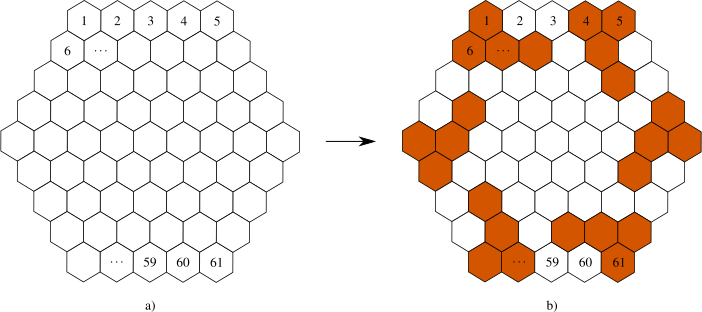
\includegraphics[scale=0.8]{Figures/ligthout3}
	\caption{Cuando se presiona la casilla $c_{_{10}}$, todas las casillas 
	adyacentes cambian su estado.}
	\label{fig:lightout3}
	\end{figure}		
	
La matriz $A_{_{61\times 61}}$ asociada al problema $A\pmb{x} = \pmb{b}$, tiene 
la forma:
\begin{equation}
A = \left[\begin{array}{ccccccccc}
D_{_5} & S_{_{56}} & & & & & & & \\
S_{_{56}}^{\top} & D_{_6} & S_{_{67}} & & & & & &\\
& S_{_{67}}^{\top} & D_{_{7}} & S_{_{78}} & & & & & \\
& & S_{_{78}}^{\top} & D_{_{8}} & S_{_{89}}  & & & & \\
& &	& S_{_{89}}^{\top} & D_{_{9}} & S_{_{89}}^{\top}   & & & \\
& & & & S_{_{89}} & D_{_{8}} & S_{_{78}}^{\top} & & \\
& & & & &  S_{_{78}} & D_{_{7}} & S_{_{67}}^{\top} & \\ 
& & & & & & S_{_{67}} & D_{_{6}} & S_{_{56}}^{\top} \\
& & & & & & & S_{_{56}} & D_{_5}
\end{array}\right],
\end{equation}
lo increíble es que ésta matriz tiene sus 61 columnas linealmente 
independientes, lo que índica que cualquier disposición inicial $\pmb{b}$ del 
juego, es combinación lineal de las columnas de $A$; es decir, dado un 
$\pmb{b}$ cualquiera, existe una estrategia ganadora $-\pmb{x}$ tal que 
$A\pmb{x} = \pmb{b}$.

Por otro lado, si se contempla la misma estructura, sólo que en esta ocasión 
cada que se presiona una casilla ella no cambia de estado, y las casillas 
adyacentes sí; la matriz $A$ sólo sufre cambios en su diagonal 
principal, tomando ceros en lugar de unos, así:

\begin{equation}
A = \left[\begin{array}{ccccccccc}
V_{_5} & S_{_{56}} & & & & & & & \\
S_{_{56}}^{\top} & V_{_6} & S_{_{67}} & & & & & &\\
& S_{_{67}}^{\top} & V_{_{7}} & S_{_{78}} & & & & & \\
& & S_{_{78}}^{\top} & V_{_{8}} & S_{_{89}}  & & & & \\
& &	& S_{_{89}}^{\top} & V_{_{9}} & S_{_{89}}^{\top}   & & & \\
& & & & S_{_{89}} & V_{_{8}} & S_{_{78}}^{\top} & & \\
& & & & &  S_{_{78}} & V_{_{7}} & S_{_{67}}^{\top} & \\ 
& & & & & & S_{_{67}} & V_{_{6}} & S_{_{56}}^{\top} \\
& & & & & & & S_{_{56}} & V_{_5}
\end{array}\right], \mbox{ con } V_{_k} =  \left[\begin{array}{ccccc}
0 & 1 & & & \\
1 & 0 & 1 & & \\
& 1 & 0 & \ddots & \\
& & \ddots & \ddots & 1 \\
& & & 1 & 0
\end{array}\right]_{k\times k}.
\end{equation}
Al poner ceros en la diagonal, los nuevos 61 vectores columnas de $A$, siguen 
siendo linealmente independientes, y esto explica que en este caso,  el juego 
también es soluble para cualquier configuración inicial. 
\end{example}

\end{section}



%\listoffigures 

%Referencia a la bibliografía: \cite[nota]{clave}
%Referenciar una entrada no citada en el documento \nocite{autor}
%Tamaño natural de las ecuaciones: $\displaystyle$  o $\displaystyle{}$
%\nocite{Anand1}
%\nocite{Vallejo1}
%\bibliographystyle{plain}
\bibliographystyle{plainnat}
\bibliography{References}

\end{document}
